\section{OrderView}

Im Order-View werden alle vom Nutzer getätigten Bestellungen angezeigt und können damit
jederzeit abgerufen werden.

\subsection{Render-Widget für Bestellungen}

Eine Bestellung wird, gleich wie ein Menü, mithlfe eines individualisierten Card-Widgets
dargestellt.
Anstatt der bekannten Informationen des Menüs werden hier die wichtigen Daten der entsprechenden
Bestellung angezeigt, dazu gehören:

\begin{itemize}
    \item das Datum der Bestellung
    \item die bestellten Waren
    \item der scanbare QR-Code der Bestellung
    \item der zu zahlende Betrag vor und nach Abzug des möglichen Rabattes
\end{itemize}

Jener QR-Code wird an der Kassa des Anbieters vom \nameref{adminclient} eingescanned, um einerseits
die bestellte Waren zu überprüfen und andererseits jene Bestellung abzuschließen und den Code
ungültig zu machen.

\begin{figure}[H]
    \centering
    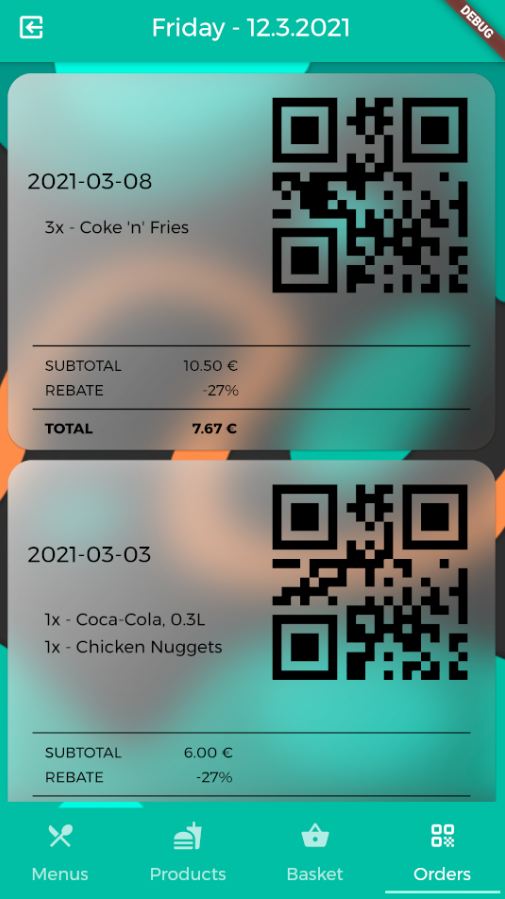
\includegraphics[width=0.40\textwidth]{images/Client/views/orderview/orderview.png}
    \caption{Order-View mit Card-Widgets für jede Bestellung}
\end{figure}
